
% !TEX encoding = UTF-8 Unicode

% This LaTeX was auto-generated from MATLAB code.
% To make changes, update the MATLAB code and republish this document.

\documentclass[12pt,final,twoside,notitlepage]{article}

% Encodage caractère et fonte
%\usepackage[utf8]{inputenc}
%\usepackage[T1]{fontenc}

% Langue: français	
\usepackage[spanish]{babel}
\usepackage{xspace}
\usepackage{fancyhdr}
\usepackage{amsmath}
\usepackage[left=3cm,right=3cm,top=2cm,bottom=6cm]{geometry}

% Utilisation de \nombre
\usepackage[autolanguage]{numprint} 

\usepackage{graphicx}
\usepackage{xcolor}
\usepackage{listings}
\definecolor{vertmatlab}{RGB}{28,160,55}
\definecolor{mauvematlab}{RGB}{155,71,239}
\definecolor{fond}{RGB}{246,246,246}
\definecolor{lightgray}{gray}{0.5}

\setlength{\parindent}{0pt}

\begin{document}
\lstset{
	language=Matlab,%
	inputencoding=utf8,%x-iso-8859-15,%
	extendedchars=true,%
	basicstyle=\footnotesize\ttfamily, % Standardschrift
	numberstyle=\tiny\color{gray},
	keywordstyle=\color{blue},
	commentstyle=\color{vertmatlab},
	stringstyle=\color{mauvematlab}\ttfamily,
	numbers=left,               % Ort der Zeilennummern
	numberstyle=\tiny\color{gray}, % Stil der Zeilennummern
	%	stepnumber=2,               % Abstand zwischen den Zeilennummern
	numbersep=5pt,              % Abstand der Nummern zum Text
	tabsize=2,                  % Groesse von Tabs
	breaklines=true,            % Zeilen werden Umgebrochen
	frame=tb,         
	%	keywordstyle=[1]\textbf,    % Stil der Keywords
	%	keywordstyle=[2]\textbf,    %
	%	keywordstyle=[3]\textbf,    %
	%	keywordstyle=[4]\textbf,   \sqrt{\sqrt{}} %
	showspaces=false,           % Leerzeichen anzeigen ?
	showtabs=false,             % Tabs anzeigen ?
	xleftmargin=17pt,
	framexleftmargin=17pt,
	framexrightmargin=0pt,
	framexbottommargin=4pt,
	backgroundcolor=\color{fond},
	showstringspaces=false,     % Leerzeichen in Strings anzeigen ?        
	literate={é}{{\'e}}1 {è}{{\`e}}1, % Accentuation française
}

\thispagestyle{fancy}
\lhead{\includegraphics[width=1.5cm]{ucr.png}}
\chead{\textbf{UNIVERSIDAD DE COSTA RICA\\FACULTAD DE CIENCIAS\\ESCUELA DE MATEMÁTICA}}
\rhead{
\includegraphics[width=4cm]{EMat.png}}

\textbf{\begin{center}
MA-0501 Análisis Numérico I\\ SOLUCIONARIO - TAREA 1\\
\end{center}}


    
    
\section*{}


\begin{par}
	El documento suministrado se publicó como $\texttt{.tex}$ con el archivo de estilo $\texttt{matlab2latex.tex}$ mediante el comando
\end{par}

\minisec{Contents}

\begin{itemize}
	
	\item Ejercicio 1)
	\item Ejercicio 2)
	\item Ejercicio 3)
	\item Ejercicio 4)
	\item Ejercicio 5)
\end{itemize}
\begin{verbatim}publish('T1_Soto_sol','format','latex','stylesheet','matlab2latex.tex')\end{verbatim}

\begin{par}
	\textbf{Respuesta Corta}
\end{par}

\begin{par}
	
1) Particularmente, no se puede utilizar a priori los métodos de
bisección ni de Newton. A priori, no se podría utilizar el método de
interación. Se considera entonces considerar la función $ h(x) = |x^2-1|e^{-x^2}$.
Esta función, comparte las mismas raices, además, se puede verificar que es una contracción
sobre $\mathbb{R}$. Ver que es una contracción es sencillo al calcular la
derivada; no se presenta la prueba. Se puede utilizar el método de
iteraciones sucesivas a la función $h$.

\end{par}

\begin{par}
	2) Al utilizar el Método de Newton para resolver la ecuación x\^{}\{100\} =0 , con un valor inicial distinto de cero, esperaría que el método no converga. Lo anterior, por cuanto alrededor de cero, la derivada de la función f(x) = x\^{}100 toma valores cercanos a 0, conforme x se toma más pequeño. En el curso se ha abordado que una de las limitaciones del Método de Newton es justamente esta. Geométricamente, la recta tangente a la curva en las valores cercanos a cero se vuelve cada vez más horizontal.
\end{par}

\begin{par}
	3) Una primera opción es calcular numéricamente las derivadas de la función en la raíz, hasta encontrar una derivada que no se anule, lo que resultaría en el cálculo de la multiplicidad. Esto puede ser computacionalmente costoso, pero es una posibilidad. Otra posiblidad sería pensar medir la rápidez convergencia de métodos como el Newton modificado.
\end{par}

\begin{par}
	4) Para precisión doble, el epsilon de la maquina viene dado por 2\^{}\{-52\}. Por lo tanto, a la iteración 52, la longitud del intervalo será de 2\^{}\{-52\}. De esta manera, a partir de realizar la iteración 52, se sobrepasaría el epsilon de la maquina. Por esta razón, no tiene sentido realizar más de 52 iteraciones.
\end{par}

\begin{par}
	
5)
Inciso a)
Dado $x_{0}$ real, se necesitan $j+1$ multiplicaciones para calcular
$ a_{j}x^{j} $, con $ 0 \leq j \leq n$. Por lo tanto, la cantidad de
multiplicaciones para evaluar $p(x_0)$ de forma directa corresponde a:

\end{par}

\begin{par}
	
\begin{equation*}
   \sum_{j=0}^{n}(j+1) = \frac{1}{2}(n+1)(n+2)
\end{equation*}

\end{par}

\begin{par}
	
Por su parte, para evaluar $p(x_0) $ directamente, se necesitan $n$ sumas.
En total, se necesitan $\frac{1}{2}(n+1)(n+2)+n$ operaciones.

\end{par}

\begin{par}
	
Inciso b) Considere la sucesión dada en el enunciado. En este caso, para
el primer paso, no se ocupa ninguna operación. Posteriormente, para el
paso $ k $, con $ 1 < k \leq n+1$, se ocupan 2 operaciones, una suma y una
multiplicación. Con lo que al final, para calcular $b_{0}$, se necesitan
un total de $2n$ operaciones.

\end{par}

\begin{par}
	Por lo tanto, para evaluar directamente el polinomio en x\_0, se ocupan más operaciones que el método del inciso b, a partir de polinomios de grado 2.
\end{par}

\begin{par}
	
Si $r_{n}$ denota el cociente
entre la cantidad de operaciones de evaluar directamente y el método del
inciso b), entonces $r_{n} = \frac{5}{4} +\frac{1}{4}n+\frac{1}{2}n = O(n)$.
Es decir, la razón se comporta casi linealmente en $ n $.

\end{par}

\begin{par}
	6) ¿Cuál es el polinomio de Lagrange de la función f(x) = x\^{}2 + 3x + 1 que interpola a $f$ en los nodos x\_\{0\} = 0, x\_1 = 1, x\_2 = 2.
\end{par}

\begin{lstlisting}
% Por cuanto se utilizan 3 nodos para interpolar a una función polinomial de
% grado 2, el polinomio de Lagrange tiene grado 2. Además, en este caso, la
% función f coincide con el polinomio de lagrange en los 3 nodos. Por unicidad,
% tiene que el polinomio de Lagrange es justamente la función  f(x) = x^2 + 3x +1
\end{lstlisting}

\begin{par}
	\textbf{Desarrollo}
\end{par}


\subsection*{Ejercicio 1)}


\begin{par}
	Inciso a) Al ejecutar el código suministrado, se obtiene para $n=10$ (note que en este caso se ejecuta el código)
\end{par}

\begin{lstlisting}
n = 10;
f = []; g = [];
f(1)=0;
f(2)=1;
for i=2:(n-1)
    f(i+1)=f(i)+f(i-1);
end

g(n)=f(n);
g(n-1)=f(n-1);
for i=(n-1):-1:2
    g(i-1)=g(i+1)-g(i);
end

% Inciso a)
% El valor máximo que se puede guardar en precisión doble en este caso,
% corresponde a
m_max = 10^16;

% Para estimar a mano el menor valor para el que se sobrepasa dicho valor
% m_max. Se utiliza la aproximación
\end{lstlisting}

\begin{par}
	
$F_{n+N} = \phi^{n}F(N)$, para $N$ lo suficientemente grande.

\end{par}

\begin{par}
	
El código del inciso, solo me corre hasta $n = 46$, por lo que este
será el valor de $ N $ utilizado. La aproximación es coherente, al considerar
el ratio F(46)/F(45).

\end{par}

\begin{par}
	De esta manera, una aproximación para el valor de $n$ máximo viene dada por:
\end{par}

\begin{lstlisting}
%phi = (1 + sqrt(5))/2;

%n_max= log(m_max/f(46))/log(phi)+46 + 1;

% Inciso c) Particularmente no pude evidenciar el fenómeno porque el código
% solamente me corre hasta  n = 46.
\end{lstlisting}


\subsection*{Ejercicio 2)}


\begin{par}
	
Inciso a) Sea dado $ b \in \mathbb{R}$, distinto de cero. Considere la
función $f(x) = 1/x - b$. Observe que dicha función es de clase $C^2 $
sobre  $\mathbb{R} \setminus \{0\}$. Particularmente, $f'(x) =
-\frac{1}{x^2}$, y $ f''(x) = - \frac{2}{x^3}$, para $x$ distinto de
cero.

\end{par}

\begin{par}
	De esta manera, dado b, se puede elegir un vecindario cerrado, sobre el cual se satisfacen las hipótesis del Teorema de Newton que garantizan la convergencia; particularmente, que la derivada de la función no se anule, y que la segunda derivada sea continua.
\end{par}

\begin{lstlisting}
% Note que dado un valor inicial  x_{0} , la fórmula de iteración de Newton
% viene dada por:
\end{lstlisting}

\begin{par}
	
\begin{equation*}
x_{n+1} = x_{n} - \frac{f(x_n)}{f'(x_n)} = 2 x_{n} - b x_{n}^2
\end{equation*}
para $ n \geq 1$.

\end{par}

\begin{par}
	Inciso b) Implementación de la función myDivision. La función implementada se encuentra al final del presente trabajo. Esta, devuelve como resultado la aproximación de la raíz, como también la sucesión de las iteraciones realizadas por el algoritmo.
\end{par}

\begin{par}
	
Inciso c) Ahora, se fija el valor $ b = \pi$. Se comprueba el
comportamiento del código para valores iniciales $x_{0}\in$
linspace(0,1,1e5).

\end{par}

\begin{par}
	Se fija el valor deseado.
\end{par}

\begin{lstlisting}
b = pi;

% Se crean los vectores para comprobar el comportamiento del código:
valores_iniciales = linspace(0,1,1e5);
valores_convergencia = nan(size(valores_iniciales));

% Se llenan los valores de convergencia con un for
for j = 1:length(valores_iniciales)
    valores_convergencia(j) = myDivision(b,valores_iniciales(j));
end

% Se procede a graficar el valor de convergencia, para los valores iniciales
% seleccionados. Se utiliza escala logarítmica en el eje x.

semilogx(valores_iniciales,valores_convergencia, 'MarkerSize', 20)
title('Convergencia en función del valor inicial')
xlabel('Valores iniciales')
ylabel('Valores de convergencia')
\end{lstlisting}

\begin{figure}[h!]
\centering
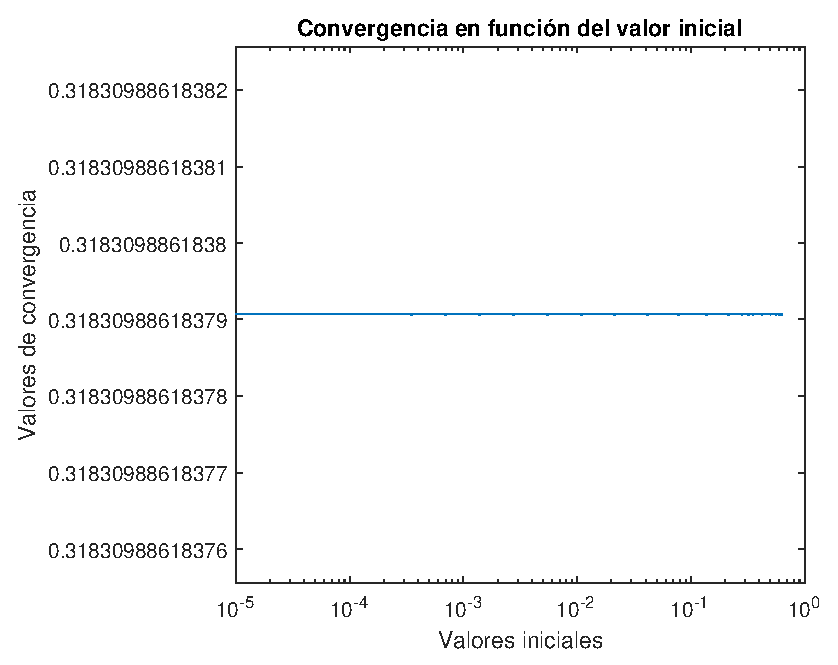
\includegraphics [width=4in]{T1_Soto_sol_01.eps}
\end{figure}

\begin{par}
	
En este caso, teóricamente, el intervalo de convergencia que garantizado
por la prueba del Teorema de Newton, es un subconjunto propio del intervalo
$(0,\frac{2/pi})$, como se observa en el gráfico anterior.

\end{par}

\begin{lstlisting}
% Inciso d)

% Particularmente, la prueba del Teorema considera la constante A,
% definida de la siguiente manera:
\end{lstlisting}

\begin{par}
	
\begin{equation*}
   A:= \max_{x,y\in I_{\delta}} \Big|\frac{f''(x)}{f'(y)}\Big| =
   2 \max_{x,y\in I_{\delta}} \Big|\frac{y^2}{x^3}\Big|
\end{equation*}

\end{par}

\begin{par}
	
Sobre un intervalo $I_{\delta}$ centrado en $1/b$, en el cual la derivada
no se anule. En este caso, se puede tomar $ \delta = 1/b - \epsilon$,
$\delta = 1/b + \epsilon$, para los casos respectivos $ b > 0$, $b <0$,
$ \epsilon > 0 $. Suponga sin perder generalidad que $ b > 0$.

\end{par}

\begin{par}
	\begin{verbatim}latex\end{verbatim} A partir de lo cual, el intervalo de convergencia garantizado por la prueba del teorema viene dado por $(\frac{1}{b}-$\ensuremath{\backslash}Tilde\{\ensuremath{\backslash}delta\}\$,\ensuremath{\backslash}frac\{1\}\{b\}+\$\ensuremath{\backslash}Tilde\{\ensuremath{\backslash}delta\}\$\$, con $\Tilde{\delta} = \min \{\frac{1}{b}, 1/A \}$ \begin{verbatim}latex\end{verbatim}
\end{par}

\begin{par}
	De esta manera,  A viene dado por
\end{par}

\begin{par}
	
\begin{equation*}
   A:= 2 \frac{(\frac{2}{b} - \varepsilon)^2}{\varepsilon^3}
\end{equation*}

\end{par}

\begin{par}
	
Numéricamente, se puede obtener el valor de $ \Tilde{\delta}$ que garantiza
el teorema de Newton, para distintos valores de $ \epsilon$.

\end{par}

\begin{par}
	
Por su parte, se puede observar que $ A > 2b $, con lo que para ser un
potencial valor inicial $x_0$, en el intervalo garantizado por el teorema,
se tendría que $\frac{1}{2b} < x_{0} < \frac{3}{2b}$; equivalentemente,
\frac{1}{2} < x_{0} b < \frac{3}{2}.

\end{par}

\begin{par}
	Las respectivas modificaciones se pueden realizar para el caso de b\ensuremath{<}0.
\end{par}


\subsection*{Ejercicio 3)}


\begin{par}
	
Considere $N_{c} = 16$ colonias de insectos. Sea $Y_{i}$ una variable
aleatoria que denota el número de insectos en cada grupo. Considere que
las variables $Y_{i}$ son independientes con distribución binomial y
parámetro $\theta$.

\end{par}

\begin{par}
	
Inciso a) Sea $ f(y_{i};\theta) $ la función de masa de probabilidad de
la variable $Y_{i}$. La función de máxima verosimilitud, denotada como
$L(y_{1},...,y_{N_c}; \theta)$, viene dada por:

\end{par}

\begin{par}
	
\begin{equation}
L(y_{1},...,y_{N_c}; \theta) = \prod_{i=1}^{N_c} f(y_{i};\theta)
=
\alpha  \theta^{y}(1-\theta)^{m}
\end{equation}

\end{par}

\begin{lstlisting}
% <latex>
% donde $ \displaystyle \alpha = \prod \binom{n_{i}}{y_{i}} $,
% $ h = \sum_{i=1}^{N_{c}}y_{i}$, $ m = \sum_{i=1}^{N_{c}}n_{i} -
% \sum_{i=1}^{N_{c}}y_{i}$. Observe que en este caso, $ h $, $ m $
% representan la cantidad total de hembras y macho en las 16 colonias,
% respectivamente.
% </latex>
\end{lstlisting}

\begin{par}
	
Se procede a encontrar el valor que maximiza la función $l(\theta)
= \log f(y_1,...,y_{N_c};\theta) $, para $\theta \in (0,1) $, cond
$y_{1},...,y_{N_c}$ dados. Observe que en este caso,

\end{par}

\begin{par}
	
\begin{equation}
l(\theta) = \log(\alpha) + h \log(\theta) + m \log(1-theta)
\end{equation}

\end{par}

\begin{par}
	
Se puede observar que dicha función es derivable, y en particular,
$ l'(\theta) = \frac{h}{\theta} - \frac{m}{1-\theta}$, para cada $ \theta
\in (0,1) $. Con el fin de maximizar dicha función, se puede observar que
el único punto crítico de la función ocurre en $ \theta = \frac{h}{h+m}$.
Particularmente, este valor maximiza la función $l(\theta)$, por cuanto
la segunda derivada de la función es negativa en su dominio.

\end{par}

\begin{lstlisting}
% Inciso b) Se cargan los datos de la distribución de insectos según
% hembras y machos, de las colonias.

T = readtable('data.txt');

% Se visualiza la tabla cargada:
disp(T);

% Inciso c)

% Se convierte el contenido de cada columna a un vector numérico a un vector
% numérico, con los siguientes comandos:

M = T.Machos ;
H = T. Hembras ;

% Se obtienen los valores de interés para el cálculo de la estimación de
% Máxima Verosimilitud.
m = sum(M);
h = sum(H);

% La estimación para el parámetro $ \theta $ es:
MLE = (h)./(m+h);

% Inciso d) Implementación del método de la secante para aproximar la
% solución numérica de la ecuación $\dfrac{dl}{d\theta} = 0$.

% El código del método de la secante se puede encontrar al final del
% presente documento.

% Se utiliza un function handle de matlab, para especificar la función
% derivada de $l(\theta)$, que es la función a la cual se quiere aproximar
% la raíz.
l_derivada = @(x) h/x - m/(1-x) ;

% Como condiciones iniciales para el método de la secante, se usan las
% siguientes:
x0 = 0.25;
x1 = 0.75;

% El valor de la raíz, con 15 decimales de exactitud viene dado por:
c = MLE;

% Se utiliza el método de la secante para obtener la raíz aproximada,
% como la sucesión de las iteraciones.
[rS,secS] = Secante(l_derivada,x0,x1) ;

% error absoluto
D_3d_iterSec_errA = abs(c-rS);
D_3d_iterSec_err = abs(c-rS)/c;

% Se observa que la aproximación obtenida con el método de la secante,
% concuerda en 16 decimales con el valor obtenido en el inciso anterior.

% Inciso e) Ahora, se utiliza también la función fsolve de MATLAB para
% aproximar la raíz deseada.

% Se utiliza la función fsolve, introduciendo dos parámetros:
% La función a la que se desea encontrar la raíz.
% El segundo parámetro corresponde al valor inicial.

[x,fval,exitflag,output,jacob] = fsolve(l_derivada,0.1);

% Al utilizar el comando anterior, entre los retornos de la función se
% encuentran:
% x: La solución dada por el algoritmo
% fval: el valor de la función en la solución encontrada

% exitflag: indica la razón por la que se detuvo el algoritmo. Toma las
% siguientes representaciones según la documentación:
% Si la ecuación fue resulta:
% 1: La optimalidad de primer orden es pequeña.
% 2: El cambio en las iteraciones es pequeña con respecto
% a la tolerancia indicada (o la default si no se indicó).
% 3: El cambio en el valor residual es menor que la
% tolerancia especificada.
% 4: La magnitud de la dirección de búsqueda es menor que la tolerancia especificada.

% Adicionalmente:
%  0: Se ha detenido por la cantidad máxima de iteraciones o evaluaciones
%  de la función.
% -1: La función de salida o la función de gráfica ha detenido el algoritmo.
% -2: Ecuación no resulta. El mensaje de salida puede tener más información
% -3: Ecuación no resulta. El radio de la región de confianza del algoritmo
% se ha vuelto demasiado pequeño

% output: especifica información sobre el proceso de optimización,
% devuelta como estructura con campos:

% Con el fin de indicar el algoritmo que se utilizó, se revisa:

disp(output);

% Se aprecia que el algoritmo utilizado fue 'trust-region-dogleg', que
% según la documentación es una modificación del método dogleg propuesto por
% Michael J. D. Powell.

D_3e_fsolve_errA = abs(x-rS);
D_3e_fsolve_err = abs(x-rS)/c;
\end{lstlisting}

\begin{lstlisting}
    Poblacion    Machos    Hembras
    _________    ______    _______

        1          11        18   
        2          22        31   
        3          27        34   
        4          29        33   
        5          24        27   
        6          29        33   
        7          25        28   
        8          26        23   
        9          38        33   
       10          14        12   
       11          23        19   
       12          31        25   
       13          20        14   
       14           6         4   
       15          34        22   
       16          12         7   

    0.4946


Equation solved.

fsolve completed because the vector of function values is near zero
as measured by the value of the function tolerance, and
the problem appears regular as measured by the gradient.

       iterations: 6
        funcCount: 14
        algorithm: 'trust-region-dogleg'
    firstorderopt: 3.3382e-10
          message: 'Equation solved.↵↵fsolve completed because the vector of function values is near zero↵as measured by the value of the function tolerance, and↵the problem appears regular as measured by the gradient.↵↵<stopping criteria details>↵↵Equation solved. The sum of squared function values, r = 1.292470e-26, is less than↵sqrt(options.FunctionTolerance) = 1.000000e-03. The relative norm of the gradient of r,↵3.338242e-10, is less than options.OptimalityTolerance = 1.000000e-06.'


\end{lstlisting}
    

\subsection*{Ejercicio 4)}


\begin{par}
	Inciso a) \begin{verbatim}latex\end{verbatim} Considere la función $g$, con criterio $g(x) = x - \frac{x^{2}-3}{2}$, para $x \in [1,2]$ \begin{verbatim}/latex\end{verbatim}
\end{par}

\begin{lstlisting}
% <latex>
% Dicha función $g$, es derivable, y su derivada viene dada por
% g'(x) = 1 - x %. De esta manera, para cada $ x \in (1,2) $, se satisface que
% $|g'(x)| < 1$. Lo que muestra que $ g $ es una contracción débil.
% </latex>
\end{lstlisting}

\begin{par}
	
Por su parte, por el cálculo de la función derivada, se observa que la
función $g$ es decreciente sobre el intervalo $ [1,2] $. Por lo tanto,
se satisface que $ g([1,2]) = [g(2),g(1)] = [\dfrac{3}{2},2]$.

\end{par}

\begin{par}
	De esta manera, por cuanto el intervalo $[1,2]$ es compacto, se tiene que la contracción débil, g, tiene un único punto fijo en [1,2], y además, la iteración simple converge a dicho punto.
\end{par}

\begin{lstlisting}
% Una prueba del resultado anterior puede ser encontrada en TKTKT.
\end{lstlisting}

\begin{par}
	
En este caso, se sencillo observar que el punto fijo en cuestión
corresponde a $ c = \sqrt{3} $.

\end{par}

\begin{lstlisting}
% Inciso b)

g = @(x) x - (x^2 -3)/2 ;

% Para la iteración, se utiliza el siguiente valor inicial:
c0 = 1.5;

% Punto fijo de la función $g$, con 16 cifras de exactitud.
c = sqrt(3); % Raíz exacta

% Se utiliza la iteración simple:
[rSimple,sSimple] = iterSimple(g,c0,80);

% Ahora, la secuencia que contiene el error relativo de cada iteración, para
% el punto inicial seleccionado, viene dada por:

D_4b_iterS_err = abs(c-sSimple)/c;

% Graficación del error relativo en función del número de iteraciones:
% En el eje y se utiliza una escala logarítmica para apreciar de mejor
% manera el comportamiento del error:

semilogy(1:80,D_4b_iterS_err,"- .")
xlabel ('Número de iteraciones')
ylabel('Error relativo')
title(['Error relativo según el número de iteraciones, con el método de ' ...
    'Iteración Simple para la función g'])

% Inciso c)

% El código que calcula la sucesión $a_{k}$ se presenta al final del
% presente documento.

[rMod,sMod] = iterModified(g,c0,80);

% Análogamente, se considera el error relativo en función del número de
% iteraciones para el nuevo método.
D_4c_iterM_err = abs(c-sMod)/c;

% Se procede a graficar los errores relativos de ambos métodos empleados
% para observar el comportamiento.

semilogy(1:80,D_4b_iterS_err,1:80,D_4c_iterM_err, ...
    "- .");
xlabel ('Número de iteraciones')
ylabel('Error relativo')
title(['Comparación de error relativo según el número de iteraciones, para ' ...
    'los métodos de iteración Simple e iteración Modificada'])
legend('Iteración Simple','Iteración modificada','Location','northeast')

% Para este caso, se observa que el método de iteración modificado genera
% una convergencia más rápida, en el sentido de una menor cantidad de
% iteraciones para obtener errores similares a los obtenidos con la
% iteración simple.

% También así, en el gráfico se observa un comportamiento decreciente
% del error hasta la iteración 32 del método de iteración modificada.
% A partir de dicha iteración, el error varía, manteniendo en general,
% una tendencia a la alza.

% Este efecto puede deberse a que cuando las iteraciones llegan a un error
% relativo bajo, el denominador del término general $a_{k}-c$ disminuye en
% menor cuantía con respecto al denominador, lo que provoca que el error
% relativo aumente conforme al número de iteraciones.
\end{lstlisting}

\begin{figure}[h!]
\centering
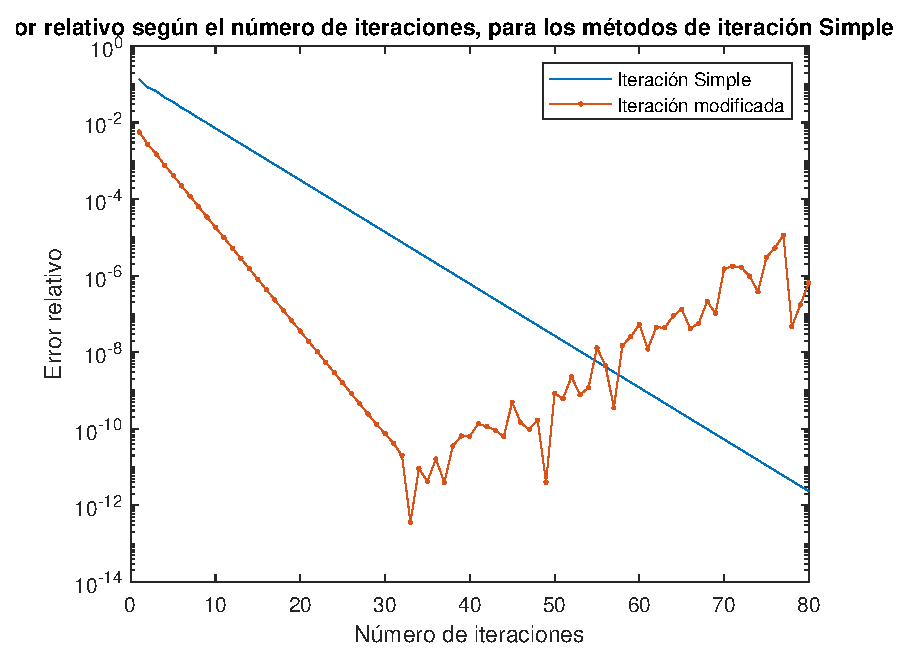
\includegraphics [width=4in]{T1_Soto_sol_02.eps}
\end{figure}


\subsection*{Ejercicio 5)}


\begin{lstlisting}
% Inciso a) Se cargan los datos del archivo .mat ejecutando el siguiente
% comando:
load('dataPolin.mat')

% Para verificar el tamaño de los vectores que fueron cargados se utilzia
% el siguiente comando:
whos("dataX","dataY")

% Se aprecia que ambos vectores tienen el mismo tamaño. Dicho tamaño se
% guarda en una variable:
n = length(dataX);

% Inciso b) Construcción del polinomio de interpolación de Lagrange que
% pasa por los puntos (x_{i},y_{i}) suministrados.

% Dada una cantidad de 80 nodos, {x_{i}}, el polinomio de Lagrange
% corresponde a la única función polinomial de grado menor o igual que 80,
% que en el nodo x_{i}, tiene el valor de y_{i}.  El grado del
% polinomio de Lagrange en este caso corresponde a 79.

% En este sentido, la función polyfit de matlab, con el comando
% polyfit(x,y,m) retorna los coeficientes de un polinomio de grado m, que
% mejor ajusta los datos de x con los de y, siendo el ajuste con el método
% de mínimos cuadrados.

% De esta manera, por la unicidad del polinomio de Lagrange, si se utiliza
% m = n-1 = 79, los coeficientes que retorna la función polyfit corresponden
% a los respectivos coeficientes del polinomio de Lagrange.

% Por lo tanto, se utiliza el siguiente comando para encontrar el polinomio
% de Lagrange, con los respectivos puntos suministrados:

pn = polyfit(dataX,dataY,n-1);
% Coeficientes polinomiales con ajuste de mínimos cuadrados, devueltos como vector.

% Inciso c) Ahora, se utiliza la función polyval para evaluar el polinomio
% que se obtuvo en el inciso anterior.

% La función polyval recibe como parámetros un vector de coeficientes, que
% corresponden a los coeficientes del polinomio que se desea evaluar.
% Además, un vector de puntos donde el polinomio es evaluado.
xx = linspace(-1,1,1e5);
yy = polyval(pn,xx);

% Se grafica el polinomio sobre el intervalo $[-1,1]$, junto con los nodos
% de interpolación.
plot(xx,yy)
hold on
scatter(dataX,dataY,15,'filled')
title('Gráfica del polinomio de interpolación de Lagrange sobre [-1,1]')
legend('Polinomio de ajuste','Nodos de interpolación','Location','northwest')
hold off
% Inciso d) Considere ahora los nodos $x_1,x_5,x_10$

data_Xmod = [-1 -0.2 0.8];
data_Ymod = [0.251083857976031,0.830828627896291,0.757200229110721];

% Nuevo polinomio:
new_p = polyfit(data_Xmod,data_Ymod,2);

xx_mod = linspace(-1,1,1e5);
yy_mod = polyval(new_p,xx_mod);

plot(xx,yy,xx_mod,yy_mod)
hold on
scatter(dataX,dataY,15,'filled')
title('Gráfica del polinomio de interpolación de Lagrange sobre [-1,1]')
legend('Polinomio de ajuste 11 nodos', 'Polinomio de ajuste 3 nodos', ...
    'Nodos de interpolación','Location','northwest')
\end{lstlisting}

\begin{lstlisting}
  Name        Size            Bytes  Class     Attributes

  dataX      11x1                88  double              
  dataY      11x1                88  double              


\end{lstlisting}
    
\begin{figure}[h!]
\centering
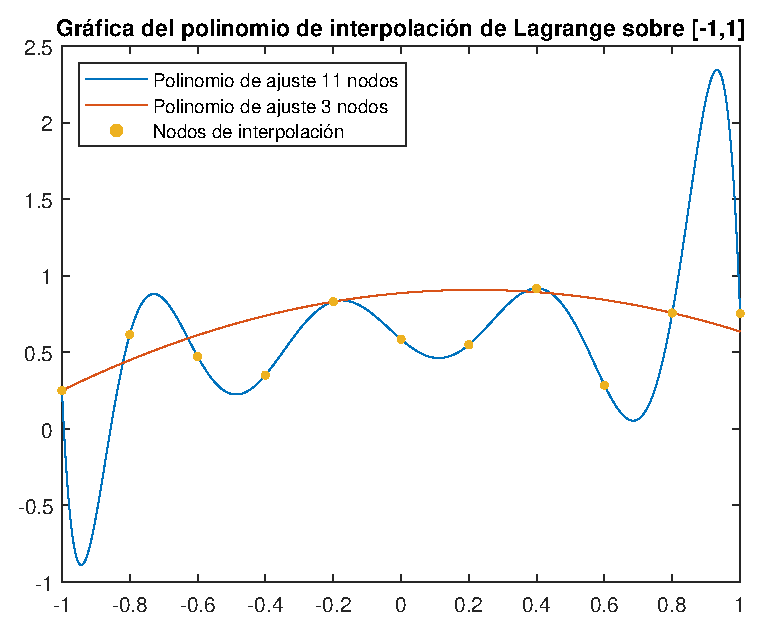
\includegraphics [width=4in]{T1_Soto_sol_03.eps}
\end{figure}

\begin{lstlisting}
close all
\end{lstlisting}

\begin{par}
	Código de Funciones: Implementación de la función del Ejercicio 2.b
\end{par}

\begin{lstlisting}
function [root,seq] = myDivision(b,x0)
  Tol = eps;
  seq = x0;
  if(abs(x0.*b - 1) < Tol.*abs(x0)) root = x0;
  else
      xNew = 2.*x0 - b.* x0^2;
      seq = [seq; xNew];
      while(abs(xNew-x0)>Tol)
        x0 = xNew;
        xNew = 2.*x0 - b.* x0^2;
        seq = [seq; xNew];
      end
      root = xNew;
  end
end

% Método de la secante. Inciso 3.d

function [root,seq] = Secante(f,c0,c1)
  Tol = 1e-8;
  iterMax = 100;
  count = 0;
  f0 = f(c0);
  f1 = f(c1);
  if(abs(f0)<Tol)     root = c0; seq = c0;
  elseif(abs(f1)<Tol) root = c1; seq = c1;
  else
      seq = zeros(iterMax,1);
      cNew = c1 - f1*(c1-c0)/(f1-f0);
      fNew = f(cNew);
      seq(1) = c0;
      seq(2) = c1;
      seq(count+3) = cNew;
      while(count<iterMax && abs(c1-c0)>Tol)
        count = count + 1;
        c0 = c1;
        c1 = cNew;
        f0 = f1;
        f1 = fNew;
        cNew = c1 - f1*(c1-c0)/(f1-f0);
        fNew = f(cNew);
        seq(count+3) = cNew;
      end
      disp(cNew)
      root = cNew;
      seq = seq(1:count+3);
  end
end

% Iteración simple, ejercicio 4.b

function [root,seq] = iterSimple(f,x0,iterMax)
Tol = 1e-8;
count = 1;
seq = zeros(iterMax,1);
seq(1) = x0;
while(count<iterMax)
    seq(count+1) = f(seq(count));
    count = count+1;
end
root = seq(end);
end

function [root,a_seq,aux_seq] = iterModified(f,x0,iterMax)
Tol = 1e-8;
k = 1;
f0 = f(x0);
aux_seq = zeros(iterMax+3,1);
aux_seq(1:3) = [x0 f0 f(f0)];
a_seq = zeros(iterMax,1);
while(k<=iterMax)
    a_k = (aux_seq(k)*aux_seq(k+2) - aux_seq(k+1)^2)./( ...
        aux_seq(k) + aux_seq(k+2) - 2*aux_seq(k+1));
    a_seq(k) = a_k;
    aux_seq(k+3) = f(aux_seq(k+2));
    k = k+1;
end
root = a_seq(end);
end
\end{lstlisting}



\end{document}
    
